\chapter{Detailed Implementation} \label{chapter:detailed_implementation}
This chapter provides an in-depth explanation of the design, architecture, and deployment of the newly implemented ASR system. It elaborates on the functionality of the system components and how they interact to achieve scalability, fault tolerance, and efficient processing.

\section{Architecture}
The new architecture of the ASR system is illustrated in Figure \ref{fig:new_architecture}. The system is designed with a microservices architecture, where each component is responsible for a specific task. 

The system consists of the following components:
\begin{itemize}
    \item \textbf{Client:} The frontend user interface that initiates transcription requests and receives the results.
    \item \textbf{NGINX Ingress Controller:} Routes incoming requests to the Live Processing Service.
    \item \textbf{Live Processing Service:} Manages the transcription tasks, interacts with the Worker Manager to allocate workers, and maintains a WebSocket connection with the client.
    \item \textbf{Worker Manager:} Allocates workers to process audio data based on the requested model and monitors the worker pods.
    \item \textbf{Worker:} Process the audio data using the specified ASR model and return the transcription results.
    \item \textbf{Message Queues:} RabbitMQ is used to decouple the communication between the Live Processing Service and the Worker.
    \item \textbf{Redis:} Stores the state information of the system, such as worker statuses and task details.
\end{itemize}

\begin{figure}[!h]
    \centering
    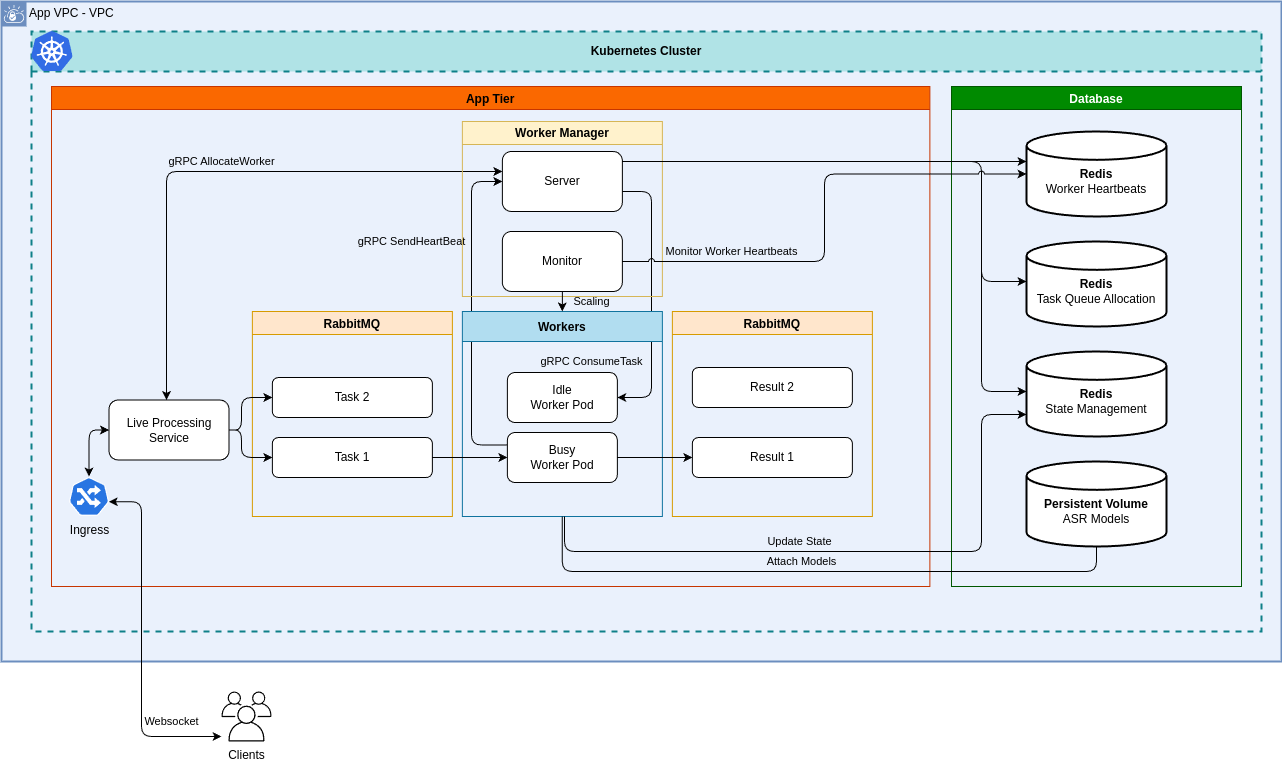
\includegraphics[width=\textwidth]{figures/new_architecture.drawio.png}
    \caption{New Architecture of the ASR System}
    \label{fig:new_architecture}
\end{figure}

\subsection{System Flow}
The sequence diagram in Figure \ref{fig:sequence_diagram} provides a detailed visualization of the ASR system's flow, showing the interactions between components during the transcription process.

\clearpage

\begin{figure}[ht]
    \centering
    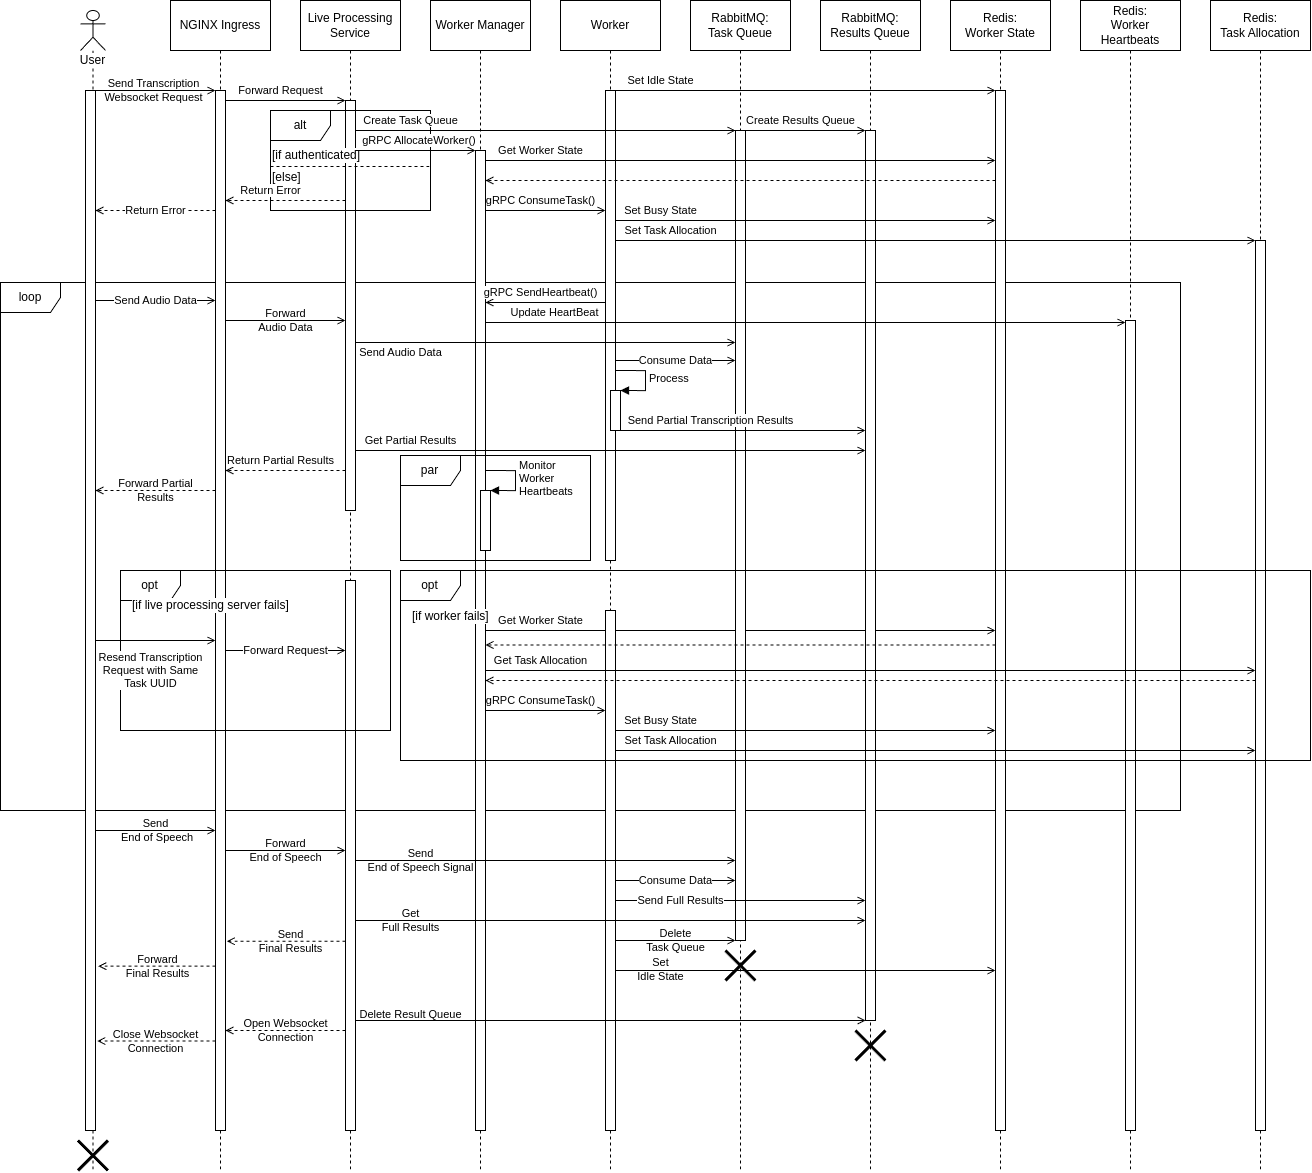
\includegraphics[width=\textwidth]{figures/sequence_diagram.drawio.png}
    \caption{Sequence Diagram of the ASR System}
    \label{fig:sequence_diagram}
\end{figure}

\subsubsection{Main Flow}
\begin{enumerate}
    \item The client establishes a WebSocket connection through the NGINX Ingress Controller to the Live Processing Service.
    \item Upon receiving the connection, the Live Processing Service creates two queues in RabbitMQ for each task:
    \begin{itemize}
        \item \texttt{task.<UUID of the task>}: Queue for the audio data to be processed.
        \item \texttt{result.<UUID of the task>}: Queue for the transcription results of the task.
    \end{itemize} 
    \item The Live Processing Service invokes the Worker Manager’s gRPC API to allocate a worker for the task.
    \item The Live Processing Service places audio data into the task queue.
    \item The Worker Manager checks the Redis database for an idle worker with the requested ASR model and assigns it to the task. The worker is notified via a gRPC call.
    \item The worker updates its state in Redis to \texttt{BUSY} and begins processing the audio data.
    \item Partial transcription results are sent to the result queue as the audio is processed.
    \item The Live Processing Service retrieves these partial results from the result queue and streams them back to the client via the WebSocket connection.
    \item Workers send periodic heartbeats to the Worker Manager to confirm their health status.
    \item When the client detects the end of speech, it notifies the Live Processing Service, which marks the task as complete by sending a special \texttt{EOS} message to the task queue.
    \item Upon processing the \texttt{EOS} message, the worker updates its state in Redis to \texttt{IDLE} and sends the final transcription result to the result queue.
    \item The Live Processing Service retrieves the final result from the result queue and delivers it to the client via WebSocket.
    \item Once all results are delivered, the WebSocket connection is closed.
\end{enumerate}

\subsubsection{Worker Failure Flow}
To maintain fault tolerance, the system detects and recovers from worker failures as follows:
\begin{enumerate}
    \item The Worker Manager detects a failure when it stops receiving heartbeats from a worker.
    \item It gets a new idle worker with the same ASR model from Redis and reassigns the task to the new worker.
    \item The new worker retrieves the pending task from the task queue, updates its state to \texttt{BUSY}, and resumes processing the audio data.
\end{enumerate}

\subsubsection{Live Processing Service Server Failure Flow}
To handle failures of the Live Processing Service:
\begin{enumerate}
    \item The client reestablishes a WebSocket connection to the Live Processing Service and resends the transcription request using the same task UUID.
    \item The Live Processing Service uses the existing task and result queues to continue processing and retrieving results, ensuring no data is lost.
\end{enumerate}

\section{Worker Manager} \label{section:worker_manager}
The Worker Manager is a key component of the system responsible for managing and coordinating worker pods. Its functionality is divided into four main responsibilities:
\begin{enumerate}
    \item \textbf{Worker Allocation:} Assigning idle workers to process audio data.
    \item \textbf{Health Monitoring:} Tracking worker health via periodic heartbeats.
    \item \textbf{Task Reassignment:} Detecting worker failures and reallocating tasks as needed.
    \item \textbf{Scaling Policy:} Dynamically adjusting the number of worker pods based on system load.
\end{enumerate}


The Worker Manager consists of two main components:
\begin{enumerate}
    \item \textbf{Worker Manager Server:} Hosts the gRPC API for worker heartbeats and worker allocation requests.
    \item \textbf{Worker Manager Monitor:} Tracks worker health and implements scaling policies.
\end{enumerate}

\subsection{Worker Manager Server}
The Worker Manager Server provides two primary gRPC APIs as shown in  Code \ref{lst:worker_manager_server}:
\begin{itemize}
    \item \texttt{AllocateWorker}: Allocates an idle worker to process audio data for a given task.
    \item \texttt{SendHeartbeat}: Receives heartbeats from workers to monitor their health status.
\end{itemize}

\begin{lstlisting}[language=Proto3, caption={Worker Manager Server gRPC Proto File}, label={lst:worker_manager_server}]
syntax = "proto3";

package worker_manager;

service WorkerManagerService {
    rpc AllocateWorker (AllocateWorkerRequest) returns (AllocateWorkerResponse);
    rpc SendHeartbeat (SendHeartbeatRequest) returns (SendHeartbeatResponse);
}

message AllocateWorkerRequest {
    string model_name = 1;
    string task_queue = 2;
}

message AllocateWorkerResponse {
    bool success = 1;
    string worker_name = 2;
    string message = 3;
}

message SendHeartbeatRequest {
    string worker_name = 1;
    string model_name = 2;
    bool final = 3;
}

message SendHeartbeatResponse {
    bool success = 1;
    string message = 2;
}
\end{lstlisting}    

\subsection{Worker Manager Monitor}
The Worker Manager Monitor is responsible for detecting worker failures and reallocating tasks. It listens for worker heartbeats and updates worker status in Redis. If a worker fails to send a heartbeat within a defined timeout, it is assumed to be unavailable, and its task is reassigned to another worker. Code \ref{lst:worker_fault_tolerance} shows the implementation of the worker fault tolerance mechanism.

\begin{lstlisting}[language=python, caption={Worker Fault Tolerance Mechanism}, label={lst:worker_fault_tolerance}]
  async def monitor_heartbeats(self):
        """
        Monitor worker heartbeats and reallocate workers if necessary.
        """
        logger.info("Monitoring worker heartbeats...")
        self.redis_client = self.redis.get_client()
        while True:
            current_time = asyncio.get_event_loop().time()
            # logger.debug(f"Current time: {current_time}")
            for worker_name, value in self.redis_client.hgetall(
                "WorkerHeartbeats"
            ).items():
                lock_key = f"lock:worker_heartbeat:{worker_name}"
                try:
                    # Acquire distributed lock
                    if self.acquire_lock(lock_key):
                        model_name, last_heartbeat = value.split(",")
                        if (
                            current_time - float(last_heartbeat)
                            > WORKER_HEARTBEAT_TIMEOUT
                        ):
                            logger.info(
                                f"Worker {worker_name} missed heartbeat. Allocating new worker."
                            )
                            try:
                                task_queue = self.redis_client.hget(
                                    "TaskAllocation", f"Worker:{worker_name}"
                                )
                            except Exception as e:
                                logger.error(f"Failed to get task queue: {str(e)}")
                                raise
                            self.allocate_worker(model_name, task_queue)
                            self.redis_client.hdel("WorkerHeartbeats", worker_name)
                            logger.info(f"Worker {worker_name} deallocated.")
                    else:
                        logger.warning(f"Failed to acquire lock for {worker_name}")
                except Exception as e:
                    logger.error(
                        f"Failed to monitor heartbeat for {worker_name}: {str(e)}"
                    )
                finally:
                    # Release distributed lock
                    self.release_lock(lock_key)

            await asyncio.sleep(WORKER_MANAGER_MONITOR_INTERVAL)
\end{lstlisting}

The Worker Manager first acquire a lock of the worker, to prevent multiple instances of the Worker Manager from processing the same worker. It then checks the last heartbeat time of the worker. If the worker has not sent a heartbeat within the specified timeout, the Worker Manager deallocates the worker and assigns a new worker to the task.

\subsubsection{Worker Scaling Policy}
The worker manager is also in charged of scaling the number of worker pods based on the current system load. A configurable \texttt{SCALING\_TARGET} is set to determine the number of idle pods required at any time. Code \ref{lst:worker_scaling} shows a snippet of the worker manager monitor's implementation.

\begin{lstlisting}[language=python, caption={Worker Scaling Policy}, label={lst:worker_scaling}]
async def monitor_and_scale():
    """
    Monitor the number of busy pods for each model and scale the statefulset up or down based on the number of idle pods.
    """

    while True:
        for model in MODELS:
            total_pods, busy_pods = get_pod_states(model)
            idle_pods = total_pods - busy_pods
            logger.info(
                f"Idle pods: {idle_pods}, Busy pods: {busy_pods}, Total pods: {total_pods}"
            )

            if idle_pods < SCALING_TARGET:
                # Scale up
                new_replicas = total_pods + (SCALING_TARGET - idle_pods)
                logger.info(f"Scaling up to {new_replicas} replicas")
                scale_statefulset(new_replicas)
            elif idle_pods > SCALING_TARGET:
                # Scale down
                new_replicas = total_pods - (idle_pods - SCALING_TARGET)
                logger.info(f"Scaling down to {new_replicas} replicas")
                scale_statefulset(new_replicas)

        # Wait for the next check
        await asyncio.sleep(CHECK_INTERVAL)
\end{lstlisting}

The system checks idle pods every \texttt{CHECK\_INTERVAL} seconds, ensuring that scaling adjustments do not occur too frequently. This is to allow for the previous scaling operation to taken effect before the next check, preventing excessive scaling activity.


\subsubsection{Health and Readiness Checks}
The Worker Manager Monitor performs health and readiness checks to ensure it is ready to handle requests. These checks are essential for maintaining the reliability and availability of the system. 

Code \ref{lst:health_check} shows the implementation of the health and readiness checks.

\begin{lstlisting}[language=python, caption={Worker Manager Monitor Health and Readiness Checks}, label={lst:health_check}]
async def healthz(request):
    return web.Response(text="OK")

async def ready(request):
    # Check Redis connection
    try:
        redis_client = WorkerManagerRedisClient().get_client()
        redis_client.ping()
    except Exception as e:
        logger.error(f"Readiness check failed: Redis connection error: {str(e)}")
        return web.Response(status=500, text="Redis connection error")

    # Check if the monitor can acquire a lock
    lock_key = "readiness_check_lock"
    if not monitor.acquire_lock(lock_key, timeout=5):
        logger.error("Readiness check failed: Unable to acquire lock")
        return web.Response(status=500, text="Unable to acquire lock")
    monitor.release_lock(lock_key)

    return web.Response(text="OK")
\end{lstlisting}

The health check (\texttt{healthz}) provides a basic indicator of whether the Worker Manager Monitor is running. It responds with an "OK" message to confirm the service is active.
The readiness check (\texttt{ready}) performs the following validations to ensure the monitor is ready to function:
\begin{enumerate}
    \item \textbf{Redis Connection:} Verifies the monitor can connect to Redis by sending a PING request.
    \item \textbf{Lock Acquisition:} Ensures the monitor can acquire and release a distributed lock, which is critical for managing shared resources.
\end{enumerate}

When deployed on Kubernetes, it continuously monitors the readiness and liveness endpoints to determine if the service is ready to receive traffic or if it needs to be restarted.

\section{Deployment}
The deployment contains two main parts: infrastructure deployment and Kubernetes cluster deployment.
\subsection{Infrastructure Deployment}
The infrastructure is deployed using Terraform, an Infrastructure-as-Code (IaC) tool that allows for the provisioning of cloud resources in a declarative manner. Terraform compares the desired state defined in configuration files with the current state of the cloud environment and makes the necessary changes to achieve the desired state.

\subsubsection{AWS Access Key and CLI Configuration}
To interact with AWS services, it is necessary to create an AWS access key. This can be done by navigating to the account credentials section in the AWS Management Console and creating an access key.

Once the access key is generated, the AWS CLI can be configured by running the command:
\begin{verbatim}
aws configure
\end{verbatim}
The CLI will prompt for the access key, secret key, region, and output format. For ease of use, a named profile can also be set up using:
\begin{verbatim}
aws configure --profile <profile-name>
\end{verbatim}
This enables switching between different AWS accounts and regions as needed.

\subsubsection{Setting Up Terraform Configuration}
Terraform is used to manage infrastructure as code. There are three main Terraform commands:
\begin{itemize}
    \item \texttt{terraform init}: Initializes the configuration, downloads necessary providers, and sets up modules.
    \item \texttt{terraform plan}: Generates an execution plan to show the changes Terraform will make to the infrastructure.
    \item \texttt{terraform apply}: Applies the changes to create or update infrastructure resources.
\end{itemize}

Code \ref{lst:terraform_plan} shows an example of the Terraform execution plan output.

\begin{lstlisting}[language=Terraform, caption={Terraform Plan Output}, label={lst:terraform_plan}]
Terraform used the selected providers to generate the following execution plan. Resource actions are indicated with the following symbols:
    + create
    <= read (data resources)
  
    Terraform will perform the following actions:
    
        # module.eks.aws_eks_addon.efs_csi_driver will be created
        + resource "aws_eks_addon" "efs_csi_driver" {
            + addon_name           = "aws-efs-csi-driver"
            + addon_version        = "v2.1.3-eksbuild.1"
            + arn                  = (known after apply)
            + cluster_name         = "ed-fyp-eks-cluster"
            + configuration_values = (known after apply)
            + created_at           = (known after apply)
            + id                   = (known after apply)
            + modified_at          = (known after apply)
            + tags_all             = {
                + "Environment" = "Development"
                + "Owner"       = "Edmund"
                + "Terraform"   = "True"
            }
        
    ... (output truncated) ...

    Plan: 37 to add, 0 to change, 0 to destroy.

\end{lstlisting}

Once we verify the plan, we can apply the changes to the infrastructure using: 
\begin{verbatim}
terraform apply
\end{verbatim}

This will update our cloud environment to match the desired state defined in the Terraform configuration files.


\subsubsection{Storing State Files in S3}
To enable collaboration among multiple developers, the Terraform state file can be stored in an Amazon S3 bucket. The state file contains the current infrastructure state and helps Terraform determine necessary changes for future deployments.


Code \ref{lst:state_bucket} shows the Terraform configuration for setting up the state bucket. We can set the bucket name and tags as variables to customize the bucket's name and attributes. This can be done by defining the variables in a separate \texttt{variables.tf} file.

\begin{lstlisting}[language=Terraform, caption={Terraform Configuration for Setting Up State Bucket}, label={lst:state_bucket}]
resource "aws_s3_bucket" "terraform_state" {
  bucket = var.bucket_name

  tags = var.tags
}

resource "aws_s3_bucket_versioning" "terraform_state" {
  bucket = aws_s3_bucket.terraform_state.id
  versioning_configuration {
    status = "Enabled"
  }
}

resource "aws_s3_bucket_public_access_block" "terraform_state" {
  bucket = aws_s3_bucket.terraform_state.id

  block_public_acls       = true
  block_public_policy     = true
  ignore_public_acls      = true
  restrict_public_buckets = true
}
\end{lstlisting}

Amazon S3 is a highly durable, scalable, and secure object storage service provided by AWS \cite{s3}. By leveraging S3 for Terraform state file storage, teams can ensure that the state file is reliably stored and accessible across all environments. This approach also promotes collaboration, consistency, and secure infrastructure management.

To prevent race conditions when multiple developers modify the infrastructure simultaneously, a DynamoDB table \cite{dynamodb} is used to store the state lock. Code \ref{lst:dynamodb_table} shows the DynamoDB table configuration.

\begin{lstlisting}[language=Terraform, caption={Terraform Configuration for Setting Up DynamoDB Table}, label={lst:dynamodb_table}]
resource "aws_dynamodb_table" "terraform-lock" {
    name = "terraform-lock"
    hash_key = "LockID"
    read_capacity = 10
    write_capacity = 10
    
    attribute {
      name = "LockID"
      type = "S"
    }
    
    tags = {
      Name = "Terraform Lock Table"
    }
}
\end{lstlisting}

The Terraform backend configuration can then be updated to use the S3 bucket and DynamoDB table, as shown in Listing~\ref{lst:backend_config}.

\begin{lstlisting}[language=Terraform, caption={Terraform Backend Configuration}, label={lst:backend_config}]
terraform {
    backend "s3" {
        bucket         = "terraform-state-bucket"
        key            = "terraform.tfstate"
        region         = "ap-southeast-1"
        dynamodb_table = "terraform-lock"
    }
}
\end{lstlisting}

\subsubsection{Deploying Terraform Resources}
The Terraform configuration files reference Song's Terraform modules \cite{song_yu}, with enhancements such as storing the Terraform state in an S3 bucket and simplifying deployment by creating an EFS CSI driver for the EFS volume. This driver allows Kubernetes pods to mount the EFS volume, enabling seamless integration.

The Terraform configuration for creating the EFS CSI driver and attaching it to the EFS volume is shown in Code \ref{lst:efs_csi_driver}. This configuration sets up the necessary IAM role, policy attachments, and the EFS CSI driver for an EKS cluster.

\begin{lstlisting}[language=Terraform, caption={Terraform Configuration for Creating EFS CSI Driver}, label={lst:efs_csi_driver},breaklines=true]
module "eks" {
  source  = "terraform-aws-modules/eks/aws"
  version = "~> 20.31"

  cluster_name    = var.cluster_name
  cluster_version = "1.31"

  vpc_id     = var.vpc_id
  subnet_ids = var.subnet_ids

  cluster_endpoint_private_access          = true
  cluster_endpoint_public_access           = true
  enable_cluster_creator_admin_permissions = true

  cluster_compute_config = {
    enabled    = true
    node_pools = ["general-purpose"]
  }
}

resource "aws_eks_addon" "efs_csi_driver" {
  cluster_name  = module.eks.cluster_name
  addon_name    = "aws-efs-csi-driver"
  addon_version = "v2.1.3-eksbuild.1"
}

resource "aws_iam_role" "efs_csi_role" {
  name = "EKS_EFS_CSI_DriverRole"
  assume_role_policy = jsonencode({
    Version = "2012-10-17"
    Statement = [
      {
        Action = [
          "sts:AssumeRoleWithWebIdentity",
        ]
        Principal = {
          Federated = "arn:aws:iam::${data.aws_caller_identity.current.account_id}: oidc-provider/${module.eks.cluster_oidc_issuer_url}"
        }
        Effect = "Allow"
        Condition = {
          StringLike = {
            "${module.eks.cluster_oidc_issuer_url}:sub" = "system:serviceaccount:kube-system:efs-csi-*",
            "${module.eks.cluster_oidc_issuer_url}:aud" = "sts.amazonaws.com"
          }
        }
      },
    ]
  })
}

resource "aws_iam_role_policy_attachment" "efs_csi_driver_policy_attachment" {
  role       = aws_iam_role.efs_csi_role.name
  policy_arn = "arn:aws:iam::aws:policy/service-role/AmazonEFSCSIDriverPolicy"
}

data "aws_caller_identity" "current" {}
\end{lstlisting}

To deploy these resources, the following commands are executed:
\begin{itemize}
    \item \texttt{terraform init}: Initializes the Terraform configuration and downloads the necessary providers and modules.
    \item \texttt{terraform plan}: Generates an execution plan that shows the changes Terraform will make to the infrastructure.
    \item \texttt{terraform apply}: Applies the changes to the infrastructure and deploys the resources.
\end{itemize}

\subsubsection{Deploying EFS and Attaching to Models}
To store the ASR models, an Elastic File System (EFS) can be deployed. The following steps outline the deployment process:
\begin{enumerate}
    \item Create an EC2 instance in a public subnet.
    \item Attach the EFS volume to the instance.
    \item Copy the ASR model files to the EFS volume.
\end{enumerate}


Code \ref{lst:ec2_setup} shows the Terraform configuration for setting up an EC2 instance and an SSH key. 

\begin{lstlisting}[caption={Terraform Configuration for Setting Up EC2 Instance}, label={lst:ec2_setup}]
# Generate new private key
resource "tls_private_key" "my_key" {
  algorithm = "RSA"
}

# Generate a key-pair with above key
resource "aws_key_pair" "key-pair" {
  key_name   = "${var.owner}-key"
  public_key = tls_private_key.my_key.public_key_openssh
}

# Saving Key Pair for ssh login for Client if needed
resource "null_resource" "save_key_pair" {
  provisioner "local-exec" {
    command = "echo  '${tls_private_key.my_key.private_key_pem}' > '${aws_key_pair.key-pair.key_name}'.pem && chmod 400 '${aws_key_pair.key-pair.key_name}'.pem"
  }
}

# create ec2 resource for mounting model
resource "aws_instance" "ec2-instance" {
  ami                         = "ami-0e48a8a6b7dc1d30b"
  instance_type               = "t2.micro"
  key_name                    = aws_key_pair.key-pair.key_name
  subnet_id                   = var.public_subnet_ids[0]
  vpc_security_group_ids      = [var.security_group_nfs_ssh]
  associate_public_ip_address = true

  tags = {
    Name = "${var.owner}-model-transfer"
  }
}
\end{lstlisting}

After the EC2 instance is created, follow these steps to transfer the model files:

\begin{enumerate}
    \item Retrieve the EC2 public IP from the AWS console.
    \item SSH into the EC2 instance using \texttt{ssh -i <key.pem> ec2-user@<public-ip>}.
\end{enumerate}

On the EC2 instance:
\begin{enumerate}
    \item \texttt{sudo mkdir -p /mnt/efs}: Create a directory to mount the EFS volume.
    \item 
        \begin{sloppypar}
            \texttt{sudo mount -t nfs4 -o nfsvers=4.1 <mount-target address>:/ /mnt/efs}: Mount the EFS volume to the directory.
        \end{sloppypar}
    \item \texttt{sudo chmod go+rw /mnt/efs}: Update the permissions of the directory to allow read and write access.

    \item 
        \begin{sloppypar}
            \texttt{scp -r -i "<private key name>.pem" \\<model-directory>@<public-ip>:/mnt/efs}: Copy the model files to the EFS volume.
        \end{sloppypar}
\end{enumerate}

\subsection{Kubernetes Cluster}
kubectl is the primary command-line tool for interacting with Kubernetes clusters. It allows users to create, update, and manage resources within the cluster. Below are some commonly used \texttt{kubectl} commands:

\begin{itemize}
    \item \texttt{kubectl apply -f <file>}: Applies the configuration defined in the YAML file to the cluster.
    \item \texttt{kubectl get <resource>}: Retrieves information about the specified resource.
    \item \texttt{kubectl describe <resource> <name>}: Provides detailed information about the specified resource.
    \item \texttt{kubectl logs <pod-name>}: Displays the logs of the specified pod.
    \item \texttt{kubectl exec -it <pod-name> -- /bin/bash}: Opens a shell in the specified pod.
    \item \texttt{kubectl delete <resource> <name>}: Deletes the specified resource.
\end{itemize}

To connect to the EKS cluster, the AWS CLI can be used to update the \texttt{kubeconfig} file with the cluster details. The following command retrieves the cluster configuration and updates the kubeconfig file:
\begin{verbatim}
aws eks --region <region> update-kubeconfig --name <cluster-name>
\end{verbatim}

Once the kubeconfig file is updated, kubectl can be used to interact with the EKS cluster.

\subsubsection{Deploying ASR System Components}
The ASR system can be deployed to the Kubernetes cluster using the Kubernetes manifest files provided in the repository. The deployment process can be initiated with the following command:
\begin{verbatim}
kubectl apply -f <file>
\end{verbatim}

The deployment includes the following components:
\begin{itemize}
    \item \textbf{Live Processing Service Deployment:} Deploys the Live Processing Service to manage transcription tasks.
    \item \textbf{Worker Manager Server and Monitor Deployment:} Deploys the Worker Manager Server to handle gRPC requests and the Worker Manager Monitor to manage worker health.
    \item \textbf{Worker Deployment:} Deploys the worker pods responsible for processing audio data.
    \item \textbf{Persistent Volume and Persistent Volume Claim:}  Defines the storage requirements for the EFS  volume used by the ASR system.
\end{itemize}



\subsubsection{Helm Charts}
\textit{To include Helm charts to deploy RabbitMQ and Redis clusters.}

\subsection{Kubernetes Dashboard}
To effectively visualize the Kubernetes cluster and monitor deployed resources, the Kubernetes Dashboard provides a graphical interface for managing the cluster, inspecting workloads, and troubleshooting issues. The dashboard allows users to view real-time metrics, manage deployments, and analyze resource utilization. Figure \ref{fig:kubernetes_dashboard} illustrates an example of the Kubernetes Dashboard.
\begin{figure}[ht]
  \centering
  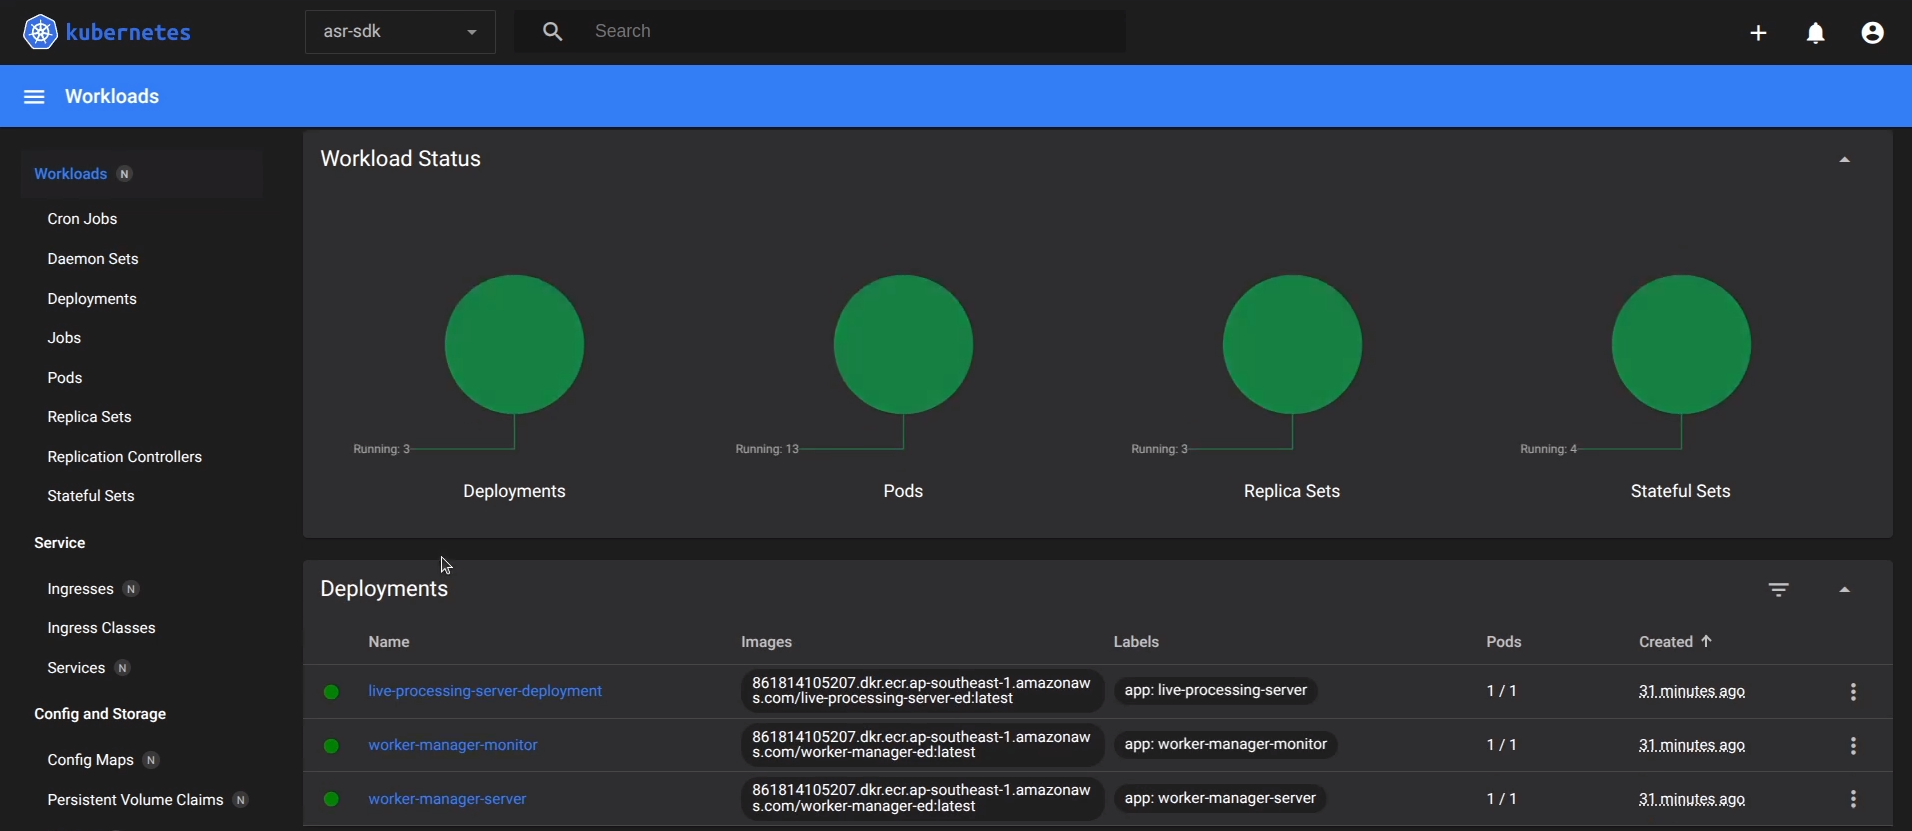
\includegraphics[width=\textwidth]{figures/kubernetes_dashboard.png}
  \caption{Kubernetes Dashboard}
  \label{fig:kubernetes_dashboard}
\end{figure}

\subsubsection{Installing the Kubernetes Dashboard}
The Kubernetes Dashboard can be installed using Helm with the following commands:

\begin{verbatim}
helm repo add kubernetes-dashboard https://kubernetes.github.io/dashboard/
helm upgrade --install kubernetes-dashboard \
  kubernetes-dashboard/kubernetes-dashboard \
  --create-namespace --namespace kubernetes-dashboard
\end{verbatim}

\subsubsection{Configuring Access and Permissions}
Before accessing the dashboard, a set of required resources must be configured, including:

\begin{itemize}
  \item \textbf{Service Account:} Grants access to the dashboard.
  \item \textbf{Cluster Role Binding:} Assigns permissions to the service account.
  \item \textbf{Secret Token:} Authenticates the dashboard.
\end{itemize}

The following Kubernetes configuration file (Code \ref{lst:k8s_dashboard_dependencies}) sets up these dependencies:

\begin{lstlisting}[language=Kubernetes, caption={Kubernetes Configuration for Setting Up Dashboard Dependencies}, label={lst:k8s_dashboard_dependencies}]
apiVersion: v1
kind: ServiceAccount
metadata:
  name: admin-user
  namespace: kubernetes-dashboard
---
apiVersion: rbac.authorization.k8s.io/v1
kind: ClusterRoleBinding
metadata:
  name: admin-user
roleRef:
  apiGroup: rbac.authorization.k8s.io
  kind: ClusterRole
  name: cluster-admin
subjects:
  - kind: ServiceAccount
    name: admin-user
    namespace: kubernetes-dashboard
---
apiVersion: v1
kind: Secret
metadata:
  name: admin-user
  namespace: kubernetes-dashboard
  annotations:
    kubernetes.io/service-account.name: "admin-user"
type: kubernetes.io/service-account-token
\end{lstlisting}

\subsubsection{Accessing the Dashboard}
Once the dashboard and necessary permissions are set up, port forwarding can be used to expose the dashboard locally:
\begin{verbatim}
kubectl -n kubernetes-dashboard port-forward \
  svc/kubernetes-dashboard-kong-proxy 8443:443
\end{verbatim}

After running this command, open a web browser and navigate to: \texttt{https://localhost:8443}.

\subsubsection{Generating Token}
To log in to the dashboard, generate an authentication token using:
\begin{verbatim}
kubectl -n kubernetes-dashboard create token admin-user
\end{verbatim}
